\documentclass[a4paper]{report}

\usepackage{verbatim}   % useful for program listings
\usepackage{color}      % use if color is used in text
\usepackage{hyperref}
\usepackage{fancyhdr}
\usepackage{pdfpages}
\usepackage{enumitem}

\lhead{\bfseries OpenBoard Release Notes}
\chead{}
\rhead{}
\lfoot{OpenBoard developer team}
\cfoot{}
\rfoot{\thepage}
\renewcommand{\headrulewidth}{0.4pt}
\renewcommand{\footrulewidth}{0.4pt}

\setlength{\textwidth}{18cm}
\setlength{\marginparwidth}{0cm}
\setlength{\oddsidemargin}{-1.cm}

\hypersetup{colorlinks=true, urlcolor=blue, linktoc=none}



\begin{document}
\thispagestyle{empty} % use if page numbers not wanted
\title{OpenBoard Release Notes}
\author{Claudio Valerio}

\maketitle
\setcounter{page}{1}
\pagenumbering{roman}
\tableofcontents


\pagestyle{fancy}
\chapter*{OpenBoard}
\addcontentsline{toc}{chapter}{OpenBoard}
\noindent 

You have between your hands the very latest version of OpenBoard. OpenBoard is a fork of the Open-Sankor\'e project version 2.00.00. \newline

The first version of OpenBoard namely 0.08.b.00 has been released the July 4th 2013. The changes were mostly related to the new application name. 

\setcounter{page}{1}
\pagenumbering{arabic}



\newpage 
\section*{ Version : 1.00.00 released the August 19, 2013}
\addcontentsline{toc}{section}{Version :1.00.00}

\begin{description}[leftmargin=!,labelwidth=\widthof{\bfseries Issue 000}]
\item[\href{http://bugs.oe-f.org/view.php?id=88 }{Issue 88}]  In mode Desktop, the label of the button OpenBoard is still in english
\item[\href{http://bugs.oe-f.org/view.php?id=5 }{Issue 5}]  Magic finger doesn't work properly with several nearby objects
\item[\href{http://bugs.oe-f.org/view.php?id=28 }{Issue 28}]  Word Uniboard appers in the first panel of the OpenBOardImporter
\item[\href{http://bugs.oe-f.org/view.php?id=22 }{Issue 22}]  Hide OpenBoard must be Cacher OpenBoard
\item[\href{http://bugs.oe-f.org/view.php?id=89 }{Issue 89}]  In Preferences, the chexbox for Importer is still in english
\end{description}
\newpage 
\section*{ Version : 0.08.b.03 released the August 15, 2013}
\addcontentsline{toc}{section}{Version :0.08.b.03}

\begin{description}[leftmargin=!,labelwidth=\widthof{\bfseries Issue 000}]
\item[\href{http://bugs.oe-f.org/view.php?id=9 }{Issue 9}]  Change home page
\item[\href{http://bugs.oe-f.org/view.php?id=62 }{Issue 62}]  Add sample of picture, video, audio, flash animations in folders
\item[\href{http://bugs.oe-f.org/view.php?id=21 }{Issue 21}]  OB proposes an update, but impossible to go to the address
\item[\href{http://bugs.oe-f.org/view.php?id=85 }{Issue 85}]  with black background, the text of the checkbox in the window for importing is invisible
\item[\href{http://bugs.oe-f.org/view.php?id=27 }{Issue 27}]  Images, sounds, videos deleted can be found in folder OB documents
\item[\href{http://bugs.oe-f.org/view.php?id=83 }{Issue 83}]  Redo button
\item[\href{http://bugs.oe-f.org/view.php?id=80 }{Issue 80}]  " does not appear correcty on ReleaseNote.pdf
\item[\href{http://bugs.oe-f.org/view.php?id=64 }{Issue 64}]  Text selected in a text box grouped with other object remains with gray background
\item[\href{http://bugs.oe-f.org/view.php?id=43 }{Issue 43}]  Z-level is not saved when copy-paste multiple objects
\item[\href{http://bugs.oe-f.org/view.php?id=81 }{Issue 81}]  Importing a pdf add a blank page 1
\item[\href{http://bugs.oe-f.org/view.php?id=49 }{Issue 49}]  An undo on z-level do not respect the last position of the item
\item[\href{http://bugs.oe-f.org/view.php?id=78 }{Issue 78}]  Z-level move up doesn't work correctly for multiple selection
\end{description}
\newpage 
\section*{ Version : 0.08.b.02 released the July 29, 2013}
\addcontentsline{toc}{section}{Version :0.08.b.02}

\begin{description}[leftmargin=!,labelwidth=\widthof{\bfseries Issue 000}]
\item[\href{http://bugs.oe-f.org/view.php?id=72 }{Issue 72}]  Pen color selection is wrong in desktop mode when the board page is black
\item[\href{http://bugs.oe-f.org/view.php?id=63 }{Issue 63}]  Using backspace in a text box when it's grouped with an other object, the group disappear.
\item[\href{http://bugs.oe-f.org/view.php?id=76 }{Issue 76}]  Add a page from another document to the actual document doesn't add anything
\item[\href{http://bugs.oe-f.org/view.php?id=27 }{Issue 27}]  Images, sounds, videos deleted can be found in folder OB documents
\item[\href{http://bugs.oe-f.org/view.php?id=46 }{Issue 46}]  Application crash sometimes  when using "Ajouter au document" or do nothing or work
\item[\href{http://bugs.oe-f.org/view.php?id=59 }{Issue 59}]  Tool takes the color of the line
\item[\href{http://bugs.oe-f.org/view.php?id=26 }{Issue 26}]  text cursor stays active event with pen selected
\item[\href{http://bugs.oe-f.org/view.php?id=29 }{Issue 29}]  Name OpenBoard doesn't appear in the file  ReleaseNotes.pdf and JournalDesModifiactions.pdf
\end{description}
\newpage 
\section*{ Version : 0.08.b.01 released the July 19, 2013}
\addcontentsline{toc}{section}{Version :0.08.b.01}

\begin{description}[leftmargin=!,labelwidth=\widthof{\bfseries Issue 000}]
\item[\href{http://bugs.oe-f.org/view.php?id=46 }{Issue 46}]  Application crash sometimes  when using "Ajouter au document" or do nothing or work
\item[\href{http://bugs.oe-f.org/view.php?id=3 }{Issue 3}]  Adapt license text of installer
\item[\href{http://bugs.oe-f.org/view.php?id=9 }{Issue 9}]  Change home page
\item[\href{http://bugs.oe-f.org/view.php?id=28 }{Issue 28}]  Word Uniboard appers in the first panel of the OpenBOardImporter
\item[\href{http://bugs.oe-f.org/view.php?id=29 }{Issue 29}]  Name OpenBoard doesn't appear in the file  ReleaseNotes.pdf and JournalDesModifiactions.pdf
\item[\href{http://bugs.oe-f.org/view.php?id=27 }{Issue 27}]  Images, sounds, videos deleted can be found in folder OB documents
\item[\href{http://bugs.oe-f.org/view.php?id=21 }{Issue 21}]  OB proposes an update, but impossible to go to the address
\item[\href{http://bugs.oe-f.org/view.php?id=62 }{Issue 62}]  Add sample of picture, video, audio, flash animations in folders
\item[\href{http://bugs.oe-f.org/view.php?id=72 }{Issue 72}]  Pen color selection is wrong in desktop mode when the board page is black
\item[\href{http://bugs.oe-f.org/view.php?id=70 }{Issue 70}]  Added PDF form the library do not appears in the navigation side frame without going to Document mode and going back to Board
\item[\href{http://bugs.oe-f.org/view.php?id=69 }{Issue 69}]  Mouse scrolling does not work without select an object.
\item[\href{http://bugs.oe-f.org/view.php?id=68 }{Issue 68}]  Mouse scrolling of the Apple Magic Mouse does not always work on Board
\item[\href{http://bugs.oe-f.org/view.php?id=66 }{Issue 66}]  Imported PDF create page with personalized format of OpenBoard. Should we can choose 16/9 or 4/3 when we import files?
\item[\href{http://bugs.oe-f.org/view.php?id=65 }{Issue 65}]  Highlighter not paint uniformly
\item[\href{http://bugs.oe-f.org/view.php?id=64 }{Issue 64}]  Text selected in a text box grouped with other object remains with gray background
\item[\href{http://bugs.oe-f.org/view.php?id=63 }{Issue 63}]  Using backspace in a text box when it's grouped with an other object, the group disappear.
\item[\href{http://bugs.oe-f.org/view.php?id=6 }{Issue 6}]  Issue with text box after resize within a group
\item[\href{http://bugs.oe-f.org/view.php?id=24 }{Issue 24}]  In the copy of objects, z-value are not respected
\item[\href{http://bugs.oe-f.org/view.php?id=26 }{Issue 26}]  text cursor stays active event with pen selected
\item[\href{http://bugs.oe-f.org/view.php?id=35 }{Issue 35}]  Magic finger doesn't select a the finest line of the pen when there is a 45° straight line on it
\item[\href{http://bugs.oe-f.org/view.php?id=42 }{Issue 42}]  Remove information when clicking item on the page
\item[\href{http://bugs.oe-f.org/view.php?id=45 }{Issue 45}]  Wrong mouse cursor appears when moving images, videos, etc  in the library
\item[\href{http://bugs.oe-f.org/view.php?id=22 }{Issue 22}]  Hide OpenBoard must be Cacher OpenBoard
\item[\href{http://bugs.oe-f.org/view.php?id=39 }{Issue 39}]  Magic Finger and undo stack
\item[\href{http://bugs.oe-f.org/view.php?id=44 }{Issue 44}]  Font size of the library text "Ajout page" and " Tout en fond"
\item[\href{http://bugs.oe-f.org/view.php?id=61 }{Issue 61}]  Can't modify the number with virtual keyboard
\item[\href{http://bugs.oe-f.org/view.php?id=60 }{Issue 60}]  Artifacts with magnifying glass
\item[\href{http://bugs.oe-f.org/view.php?id=59 }{Issue 59}]  Tool takes the color of the line
\item[\href{http://bugs.oe-f.org/view.php?id=56 }{Issue 56}]  Cant' use trap web
\item[\href{http://bugs.oe-f.org/view.php?id=55 }{Issue 55}]  Can't use the virtual keyboard with trap content
\item[\href{http://bugs.oe-f.org/view.php?id=54 }{Issue 54}]  Can't hide tools in web mode
\item[\href{http://bugs.oe-f.org/view.php?id=51 }{Issue 51}]  Moving an item display artifacts
\item[\href{http://bugs.oe-f.org/view.php?id=49 }{Issue 49}]  An undo on z-level do not respect the last position of the item
\item[\href{http://bugs.oe-f.org/view.php?id=43 }{Issue 43}]  Z-level is not saved when copy-paste multiple objects
\item[\href{http://bugs.oe-f.org/view.php?id=40 }{Issue 40}]  Flash doesn't appear in Podcast
\item[\href{http://bugs.oe-f.org/view.php?id=37 }{Issue 37}]  Mode Desktop, impossible to use with stylet and Wacom PL720
\item[\href{http://bugs.oe-f.org/view.php?id=75 }{Issue 75}]  Size of image not respected when using board capture and send it to library
\item[\href{http://bugs.oe-f.org/view.php?id=74 }{Issue 74}]  Impossible to switch to greek keyboard language by the floating keyboard
\item[\href{http://bugs.oe-f.org/view.php?id=47 }{Issue 47}]  Rectangular forms are not well draw in the upper left corner
\item[\href{http://bugs.oe-f.org/view.php?id=8 }{Issue 8}]  Automatic opening of the virtual keyboard when you click on a text field
\item[\href{http://bugs.oe-f.org/view.php?id=16 }{Issue 16}]  Using the stylus on a table PC to draw creats a delay before the detection of the movement
\item[\href{http://bugs.oe-f.org/view.php?id=48 }{Issue 48}]  Impossible to resize 2 items selected - Is it normal ?
\item[\href{http://bugs.oe-f.org/view.php?id=52 }{Issue 52}]  Unable to copy and paste text from url field and search field
\item[\href{http://bugs.oe-f.org/view.php?id=2 }{Issue 2}]  Installer/App need to be signed
\item[\href{http://bugs.oe-f.org/view.php?id=57 }{Issue 57}]  Impossible to import an .iwb file
\end{description}


\chapter*{Open-Sankore}
\addcontentsline{toc}{chapter}{Open-Sankore}
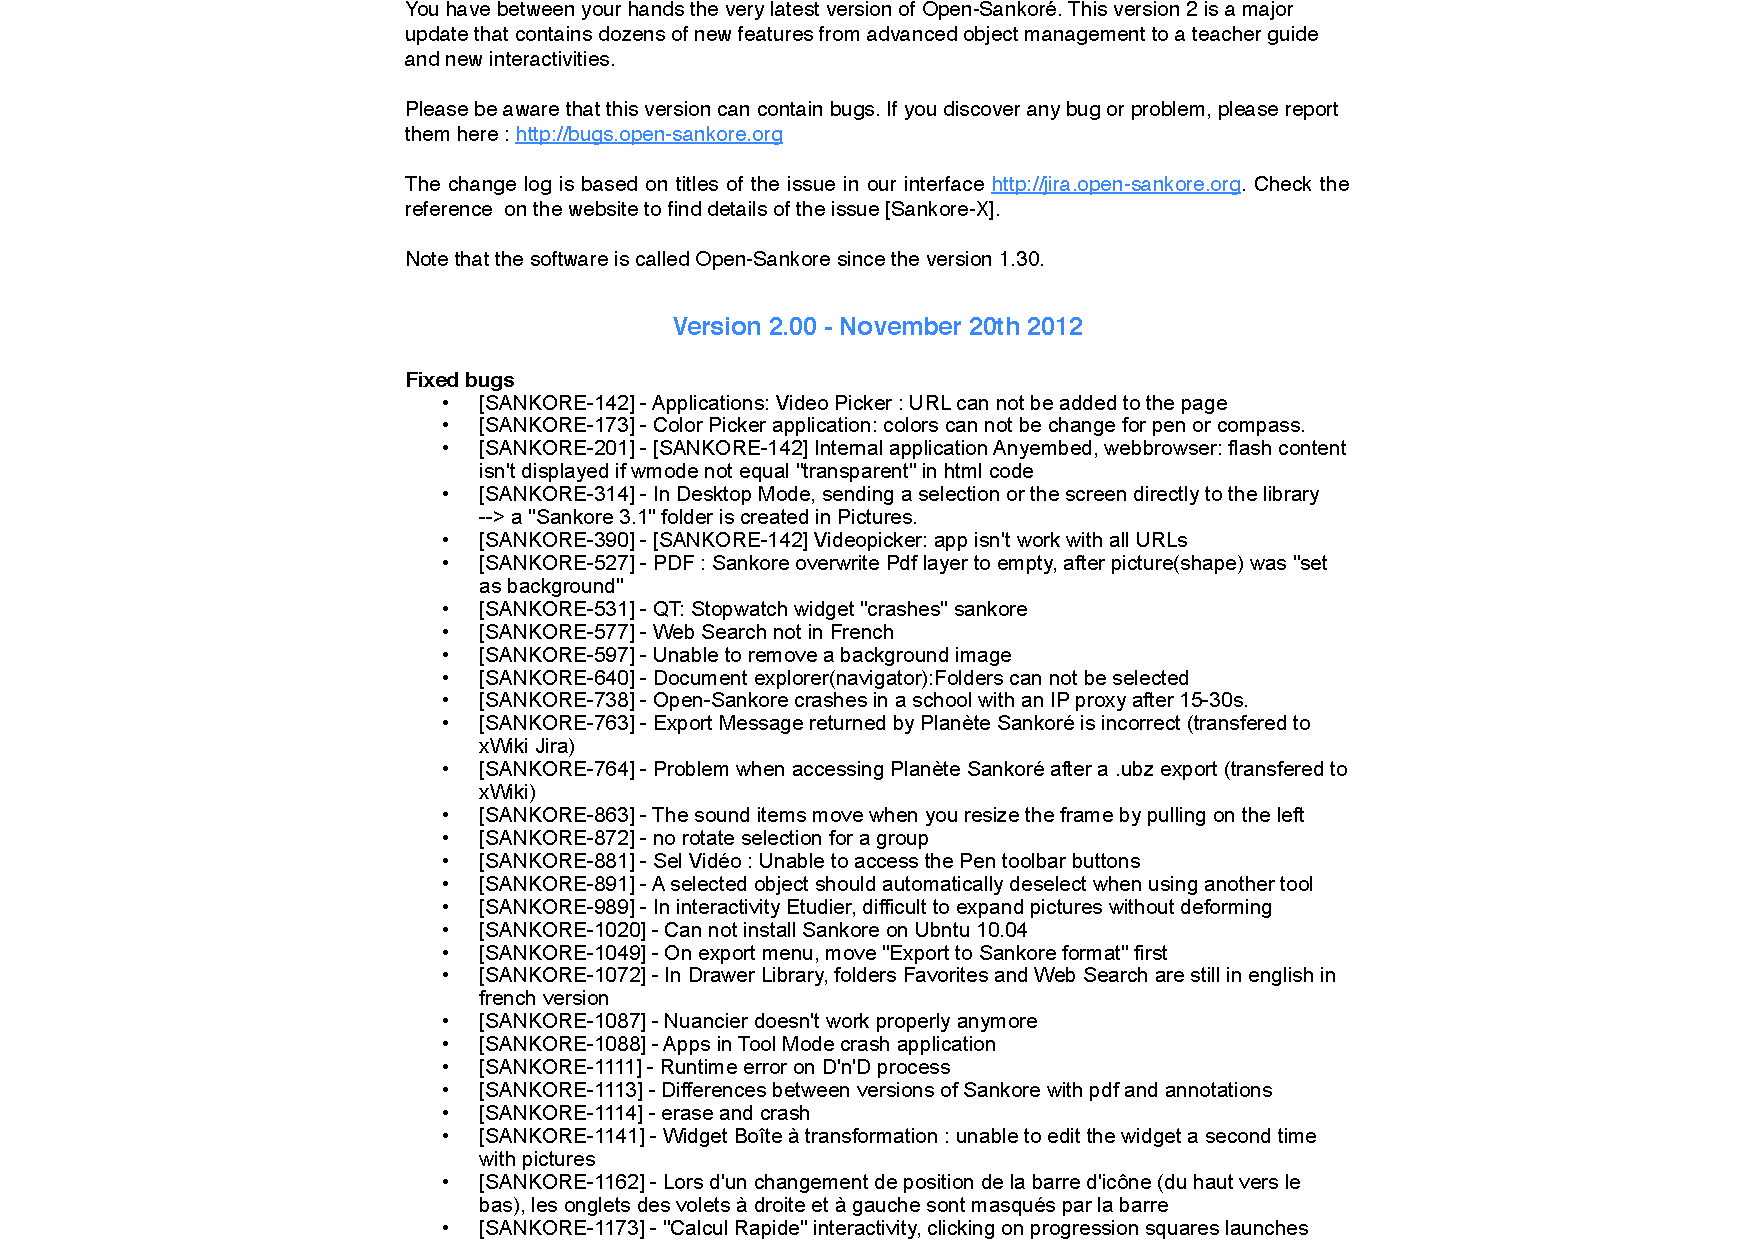
\includepdf[pages={-}]{sankore.pdf}
\end{document}